\section{پیش‌نمونه سازی
چیست}\label{ux67eux6ccux634ux646ux645ux648ux646ux647-ux633ux627ux632ux6cc-ux686ux6ccux633ux62a}

اکنون که شما بصورت اولیه میدانید که منظور من از آن \textbf{چیز}
\emph{درست} چیست، ما می‌توانیم مقدمه قابل قبول درباره پیش‌نمونه سازی
داشته باشیم. بهترین راه برای این کار بررسی دو داستانی است که من را به
فکر این موضوع انداخت: «آزمایش» تبدیل گفتار به متن آی بی ام و «آزمایش»
پالم پایلوت.

\section{آزمایش تبدیل گفتار به متن آی بی
ام}\label{ux622ux632ux645ux627ux6ccux634-ux62aux628ux62fux6ccux644-ux6afux641ux62aux627ux631-ux628ux647-ux645ux62aux646-ux622ux6cc-ux628ux6cc-ux627ux645}

اولین بار من این داستان را چند سال پیش در ارائه‌ای در یکی از کنفرانس‌های
نرم‌افزار شنیدم. من مطمئن نیستم که تعاریف من از ماجراها چقدر دقیق است.
ممکن است من برخی از جزئیات را اشتباه دریافته باشم، اما نتیجه اخلاقی
ماجرا بسیار از جزئیات آن مهم‌تر است. با در نظر گرفتن این موضوع، این
داستانی است که من بخاطر می‌آورم.

چند دهه پیش، قبل از عصر اینترنت و حتی قبل از طلوع کامپیوترهای شخصی، آی
بی ام بخاطر ماشین تحریر و کامپیوترهای \lr{Mainframe} اش مشهور بود. در آن
زمان تایپ‌کردن یکی از ویژگی‌هایی بود که افراد کمی آنرا بخوبی انجام
می‌دادند و بیشتر آنها منشی، نویسنده و برخی از برنامه‌نویسان بودند. بیشتر
افراد از یک انگشت برای تایپ استفاده می‌کردند که کند و ناکارآمد بود.

آی بی ام درست در نقطه‌ای قرار داشت که بتواند از تجربه خود در بازار
کامپیوتر و ماشین تحریر استفاده کرده یک ماشین تبدیل گفتار به متن توسعه
دهد. این ابزار به افراد اجازه میداد که در یک میکروفن صحبت کنند و متن
بصورت «جادویی» روی صفحه نمایش ظاهر شود و دیگر نیازی به تایپ کردن نباشد.
این دستگاه پتانسیل زیادی برای کسب درآمد برای آی بی ام داشت و \emph{ریسک
بزرگ} روی این موضوع برای شرکت قابل قبول به نظر میرسید.

اما در این میان چندین اشکال بزرگ وجود داشت. کامپیوترها در آن زمان کم
قدرت تر و بسیار گرانتر از امروزه بوده و تبدیل گفتار به متن نیاز به
پردازش زیادی داشت. همچنین، با داشتن قدرت محاسباتی کافی، تبدیل گفتار به
متن یک مساله بسیار سخت علوم کامپیوتر بوده و هست. دست و پنچه نرم کردن با
این مساله نیاز به سرمایه‌گذاری عظیم -حتی برای آی بی ام- و صرف سال‌های
زیاد برای تحقیق داشت. اما همه به این دستگاه نیاز داشتند. آیا واقعا این
یک موفقیت واضح خواهد بود یا نه؟

برخی در آی بی ام با حرف افرادی که میگفتند که مردم تبدیل گفتار به متن
«نیاز داشته و قطعا آنرا خریداری نموده و استفاده میکنند» قانع نشده بودند
و فکر نمی‌کردند این دستگاه به موفقیت برسد. آنها از این می‌ترسیند که
سال‌ها تحقیق و سرمایه شرکت صرف توسعه دستگاهی شود که اندکی آنرا میخرند که
این یک فاجعه در کسب و کار است. به زبان پیش‌نمونه سازی آنها مطمئن نبودند
که تبدیل گفتار به متن یک \textbf{چیز} \emph{درست} است. همچنین، مردم تا
کنون از تبدیل گفتار به متن استفاده نکرده بودند ، پس آنها نمی‌توانستند
بصورت قطعی بدانند که کسی به این دستگاه نیاز دارد یا نه؟ آی بی ام نیاز به
بررسی قابلیت ماندگاری این دستگاه در کسب و کار داشت اما ساختن حتی یک
نمونه اولیه نیاز به سال‌ها زمان داشت. آنها بجای آن یک آزمایش مبتکرانه
طراحی کردند.

آنها مشتریان بالقوه دستگاه تبدیل گفتار به متن خود را که به نظر آنها قطعا
خریدار این دستگاه بودند در اتاقی با یک کامپیوتر، یک میکروفن و یک صفحه
نمایش بدون کیبرد قرار دادند. به آنها گفتند که یک ماشین تبدیل خودکار
گفتار به متن ساخته‌اند و میخواهند ارزیابی کنند که آیا مردم از استفاده از
آن لذت میبرند یا نه. وقتی آزمایش دهنده‌ها شروع به صحبت در میکروفن کردند
متن آنها تقریبا بی درنگ و بدون خطا روی صفحه نمایش ظاهر می‌شد! کاربران
تحت تاثیر قرار گرفته بودند. این برای واقعی بودن خیلی خوب بود که بعدا
معلوم شد واقعی نبوده است.

اتفاق پشت صحنه که این آزمایش را مبتکرانه میکند این بود که ماشین تبدیل
گفتار به متن حتی یک نمونه اولیه نبود. کامپیوتر موجود در اتاق خالی ساختگی
بود. در اتاق کناری یک تایپیست کارآزموده در حال گوش کردن به صدای کاربر
بود و با استفاده از کیبرد صحبت‌های او را تایپ و دستورات او را اجرا
میکرد. هرچه تایپیست تایپ میکرد روی صفحه نمایش کاربر نشان داده می‌شد.
صحنه سازی انجام شده به گونه‌ای بود که کاربر قانع میشد که خروجی روی صفحه
نمایش خروجی دستگاه تبدیل گفتار به متن است.

اما آی بی ام از این آزمایش چه یاد گرفت؟

این چیزی است که من شنیده‌ام: بعد از تاثیر اولیه بوسیله «تکنولوژی»،
بسیاری از افرادی که خریدار این سیستم بودند پس از چند ساعت کار با این
سیستم نظرشان عوض شد. گفتن چندین خط متن از طریق گفتار در کامپیوتر حتی با
استفاده تبدیل تقریبا بدون نقص و سریع توسط تایپیست هم دارای مشکلات زیادی
بود: گلوی افراد بر اثر صحبت زیاد خشک میشد، محیط کار پر از هم همه میشد و
به درد موارد محرمانه نمی‌خورد.

براساس نتایج این آزمایش، آی بی ام باز هم در تبدیل گفتار به متن سرمایه
گذاری نمود اما در مقیاسی به مراتب کمتر - آنها با این سرمایه‌گذاری روی
\emph{اعتبار شرکت قمار} نکردند.

اینطور به نظر میرسد که این یک تصمیم درست در کسب و کار بوده است. کیبردها
نشان‌داده اند که در مورد وارد کردن متن به سختی شکست می‌خورند. سی سال پیش
مردم نمی‌توانستند تایپ کنند اما اکنون در هر دفتر (یا کافی شاپی) افراد
مختلف در سنین و شغل‌های مختلف را می‌بینید که در حال تایپ روی لپ‌تاپ‌های
خود هستند. در دستگاه‌هایی که کیبرد با سایز استاندارد غیر قابل استفاده
است همانند موبایل‌ها، تبدیل گفتار به متن میتواند یک \textbf{چیز}
\emph{درست} باشد اما در غیر اینصورت هنوز بایستی کیبرد را شکست بدهید.
کیبرد قطعا یک \textbf{چیز} \emph{درست} است.

راهبرد آی بی ام مبتکرانه بود، اما شما به آن چه عنوانی می‌دهید. صحنه سازی
تبدیل گفتار به متن به کمک یک تایپیست قطعا یک «نمونه اولیه مناسب» نیست
مگر اینکه قصد داشته باشید که واقعا یک تایپیست زنده را درون یک کامپیوتر
جا بدهید. آنها یک نمونه اولیه از تبدیل گفتار به متن نساختند، بلکه
\emph{وانمود} کردند که یک نمونه اولیه تبدیل گفتار به متن داشته و از آن
به منظور دریافت عکس‌العمل مشتری به محصول استفاده کردند. در این حالت آنها
امکان جمع آوری اطلاعات با ارزش بازار را براساس استفاده واقعی به جای نظر
افراد داشتند، همچنین سرمایه‌گذاری مالی و زمانی کمی انجام دادند.

به نظر من این راهبرد بسیار ارزشمند و جالب است، و این روش به اندازه کافی
از ساختن نمونه اولیه متفاوت بوده که نام خاصی به خودش اختصاص دهد (که
بیشتر در مورد آن صحبت خواهم کرد). همچنین این روش ارزش بررسی را دارد. اما
قبل از ادامه سعی به یافتن مثال‌های دیگر در این زمینه کردم که یک مثال
عالی پیدا کردم.

\section{آزمایش پالم
پایلوت}\label{ux622ux632ux645ux627ux6ccux634-ux67eux627ux644ux645-ux67eux627ux6ccux644ux648ux62a}

آزمایش تبدیل گفتار به متن آی بی ام من را به فکر در مورد مفهوم پیش‌نمونه
سازی واداشت، اما این مثال، من را قانع کرد که این روش ارزش پیگیری را
دارد.

پالم پایلوت در سال 1996 معرفی شد که به اندازه کف دست بوده و چهار عملیات
اصلی را انجام میداد: تقویم، دفتر تلفن، لیست کارهای روزمره و یادداشت
برداری ساده. پالم پایلوت اولین نمونه موفق دستیاران شخصی بود، اما جف
هاوکینز -یکی از بنیانگذاران پالم و مخترع پایلوت- به موفقیت دستیارهای
شخصی مطمئن نبود. برعکس باتوجه به مقاله سال 1998 در مجله تایمز(تاکیدها را
من اضافه کرده ام):

\begin{quote}
هاوکینگ ۴۰ ساله، مدیر تکنولوژی پالم و مخترع پالم، یکی از اولین
کامپیوترهای قابل حمل به نام گریدپد را ده سال پیش ساخته است. این کامپیوتر
یک \textbf{پدیده اعجاز انگیز مهندسی اما یک شکست تجاری} بود به خاطر اینکه
به نظر او هنوز بسیار بزرگ بود. وقتی همکاران او از او پرسیدند که
کامپیوترهای جدید چه اندازه ای باید باشد \textbf{برای اطمینان از اینکه
این اشتباه را دوباره تکرار نکند} برای آنها جواب آماده‌ای داشت: «بیایید
سایز جیب لباس را \textbf{آزمایش کنیم}»
\end{quote}

\begin{quote}
او به گاراژ خود بازگشت و یک تکه چوب را به اندازه سایز جیب لباس خود برید.
سپس او این تکه چوب را در ماه‌های متمادی حمل کرد و \textbf{تظاهر} کرد که
آن تکه چوب واقعا یک کامپیوتر است. آیا او برای ناهار چهار شنبه آزاد بود؟
هاوکینز آن تکه چوب را از جیبش خارج میکرد و انگار که دارد برنامه زمانی
خود را چک میکند آنرا میفشرد. اگر او به شماره تلفنی نیاز داشت، او
\textbf{تظاهر} به پیدا کردن آنرا در قطعه چوب میکرد. معمولا او طراحی
ظاهری متفاوتی را با چینش دکمه‌های متفاوت رو کاغذ پرینت میکرد و با
چسباندن آنها روی چوب طراحی جدید را امتحان میکرد.
\end{quote}

این عکس پیش‌نمونه‌ای است که جف آنرا ساخته است(شما میتوانید نمونه‌های
بیشتری در موزه تاریخچه کامپیوتر در مانیتن ویوو کالیفرنیا پیدا کنید).

\begin{figure}[htbp]
\centering
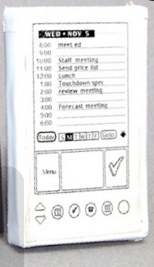
\includegraphics{palmpilot.png}
\caption{پیش نمونه پالم پایلوت}
\end{figure}

من فقط میتوانم عکس العمل دیگران را هنگامی که هاوکینز آن تکه چوب را از
جیب خود بیرون می‌آورد و آنرا همانند یک کامپیوتر فعال میفشرد تصور کنم.
آنها فکر میکردند که او دیوانه شده است. اما نه او بسیار باهوش بود. آن تکه
چوب به همراه دکمه‌های پرینت‌شده هاوکینز را به این نتیجه رساند که او راه
درستی را آمده است. او برای اولین و مهمترین سوال پاسخی یافته بود: «اگه من
یک پایلوت داشتم، آیا آنرا با خود حمل کرده و از \textbf{آن چیز} استفاده
میکردم؟» و جواب قطعا «بله» بود و او میدانست که \textbf{چیز} \emph{درست}
را یافته است. اکنون او می‌توانست روی سوالات بعدی تمرکز کند مانند: آیا
می‌توانم آنرا کوچک درست کنیم؟ ساخت آن چقدر هزینه خواهد برد؟ عمر باتری‌ها
چقدر خواهد بود؟ اکنون زمان ساخت یک «نمونه اولیه مناسب» رسیده بود.

پالم پایلوت تنها موفق نبود بکله یک موفقیت بسیار بزرگ با تاثیر عظیم بود.
پایلوت جد تمامی تلفن‌های هوشمند امروزی است. این محصول تنها از تکه چوبی
شروع شد همانند پینوکیو.

\section{وانمود کنید قبل از اینکه
بسازید}\label{ux648ux627ux646ux645ux648ux62f-ux6a9ux646ux6ccux62f-ux642ux628ux644-ux627ux632-ux627ux6ccux646ux6a9ux647-ux628ux633ux627ux632ux6ccux62f}

داستان‌های تبدیل گفتار به متن و پالم پایلوت چیزهای مشترک بسیاری دراند.

\begin{quote}
هر دو تیم شک‌های زیادی درباره سودمندی و قابلیت استفاده و پذیرش ایده خود
داشتند. هر دو ایده جالب بوده، درست به نظر رسیده و مساله‌ای را حل
می‌کردند. اما آیا آنها یک \textbf{چیز} \emph{درست} بودند؟ آیا مردم واقعا
از آنها استفاده می‌کردند؟ جف هاوکینز حتی سالهای زیادی را برای توسعه
محصول (گریدپد) که «پدیده اعجاز انگیز مهندسی اما یک شکست تجاری بود»، از
دست داده بود(یک \textbf{چیز} \emph{غلط}) و تصمیم داشت که «این اشتباه را
دوباره تکرار نکند».
\end{quote}

\begin{quote}
بخاطر شکشان هر دو تیم میخواستند کاربردپذیری و سودمندی ایده‌هایشان را با
ساختن یک نمونه اولیه آزمایش کنند. همچنین قبل از اینکه شروع به توسعه
محصول کنند، بازخوردهای \emph{استفاده واقعی از محصول}(بجای \emph{نظرات در
مورد محصول}) را جمع آوری کنند.
\end{quote}

\begin{quote}
در هر دو آزمایش اما توسعه حتی یک «نمونه اولیه مناسب»(نسخه خام ولی
عملیاتی محصول نهایی) زمان بسیار و سرمایه‌گذاری قابل توجهی برای تحقیق و
توسعه نیاز داشت.
\end{quote}

\begin{quote}
راه حل آنها برای مشکل «نمونه اولیه مناسب» این بود که \emph{تظاهر} به
داشتن یک چنین نمونه اولیه‌ای کنند. در مثال تبدیل گفتار به متن، سخت افزار
و نرم‌افزار با کمی حیله گری جایگزین شده بود و در پالم پایلوت با قوه تخیل
هاوکینز جایگزین شده بود. \emph{وانمود کنید قبل از اینکه آنرا بسازید}
\end{quote}

به نظر من این دو داستان بخاطر تفاوت بسیار از آنچه افراد و شرکت‌ها بصورت
معمول در پیگیری ایده‌های نوشان انجام می‌دهند قابل توجه و موثر بودند.
بیشتر مردم عاشق ایده‌ی شان می‌شوند(آن \textbf{چیز} آنها) و فرض می‌کنند
که آن \textbf{چیز} موفق خواهد بود(آن \textbf{چیز} \emph{درست}) پس شروع
به ساختن آن می‌کنند. آنها پیش از موعد شروع به تمرکز و سرمایه‌گذاری روی
چیزهای غلط در زمان غلط می‌کنند. بصورت دقیق‌تر، آنها بیشتر از نیاز و پیش
از موعد روی توسعه اولین نسخه محصول خود که دارای ویژگی‌های زیاد،
کارکردهای بیش از حد و «رنگ و لعاب» بیش از حد نیاز است، سرمایه‌گذاری
می‌کنند. آنها پیش‌فرضشان بر این است که مردم آنرا خواهند خواست. در بسیاری
از موارد، این پیش‌فرض ها و فرضیات هم غلط و هم پر هزینه از کار در می
آیند.

\section{پیش‌نمونه سازی: کلمه بوجود
آمد}\label{ux67eux6ccux634ux646ux645ux648ux646ux647-ux633ux627ux632ux6cc-ux6a9ux644ux645ux647-ux628ux648ux62cux648ux62f-ux622ux645ux62f}

من هرچه بیشتر در مورد تبدیل آزمایش متن به گفتار و پالم پایلوت فکر
میکردم، بیشتر قانع می‌شدم که کاری که آن تیم‌ها انجام دادند نه تنها
هوشمندانه بودند بلکه این یک مرحله ضروری در روند توسعه یک محصول جدید و
خلاقانه است. مرحله‌ای که اکثر افراد آنرا از قلم انداخته و اغلب منجر یه
پرداخت هزینه زیادی بخاطر این نادیده گرفتن می شوند.

در طول چند ماه، من این دو داستان را با گروه قابل توجهی از دوستان،
همکاران، کارآفرینان، سرمایه‌گذاران پر ریسک، مهندسان و مدیران محصول به
اشتراک گذاشتم. با تعجب، هیچکدام از آنها این مثال‌ها را قبلا نشنیده
بودند. همه آنها، اما تحت تاثیر راه حل هوشمندانه «وانمود کنید قبل از
اینکه آنرا بسازید» قرار گرفته بودند و برخی از آنها حتی به پیشانی خود
زدند و چیزهایی شبیه «کاش من به همچنین روشی عمل میکردم قبل از اینکه
سال‌ها و میلیون‌ها دلار را روی ایده آخرم از دست میدادم.» گفتند.

من پی‌بردم که بصورت اتفاقی به موضوع مهم و ارزشمندی -با اینکه جدید یا بکر
نبود- برخورده‌ام که مشهور نبوده و از آن بصورت گسترده استفاده نمی‌شود.
اما این موضوع اسمی نداشت که آنرا توصیف کند و من فکر کردم که این موضوع
برای شناخته شدن، مورد بررسی قرار گرفتن و استفاده نیاز به نامی دارد. پس
من شروع به فکر در مورد اسم برای این موضوع کردم(توجه: من در زمان شروع فکر
در این مورد پیش‌نمونه سازی من در مورد \emph{ماشین استارت آپ ناب} که توسط
اریک ریس و \emph{کمینه محصول قابل قبول}\footnote{\lr{Minimum}
  \lr{Viable} \lr{Product}} اطلاعاتی نداشتم. بیشتر در مورد رابطه بین
پیش‌نمونه سازی و کمینه محصول قابل قبول در بعد آورده می‌شود).

از آنجایی که نقطه اصلی و کلیدی هر دو مثال \emph{تظاهر} بود (کارمندان آی
بی ام تظاهر به ساختن ماشین تبدیل گفتار به متن کردند و جف هاوکینز تظاهر
به داشتن پالم پایلوت در جیب لباس خود می‌کرد) اولین کلمه‌ای که به ذهن
میرسید\_‌نمونه اولیه متظاهر\_ است ایش! تلاش دوم من برای پیدا کردن نام
حتی بدتر بود. از آنجایی که ایده‌ اصلی تست سریع ایده \emph{قبل} از گذاشتن
سرمایه کافی برای نمونه اولیه مناسب است، من به کلمه \emph{پیش نمونه اولیه
سازی} رسیدم، ایش ایش! خوشبختانه این دو کلمه بد نطفه یک کلمه بهتر را
ایجاد کردند. با حذف برخی از کلمات، من به \emph{پیش‌نمونه سازی} رسیدم.
خیلی خوب. چیزهایی که در روند پیش‌نمونه سازی تولید می‌شوند(مانند قطعه چوب
هاوکینز) پیش‌نمونه گفته می‌شوند.

من از اصطلاحات پیش‌نمونه‌سازی\footnote{\lr{Pretotyping}} و
پیش‌نمونه\footnote{\lr{Pretotype}} خوشم می‌آید اما آیا من اولین نفری
هستم که از این کلمه استفاده می‌کنم؟ ممکن است تا الان کسی از این اصطلاحات
استفاده کرده باشد و «حقوقی» را برای استفاده از آن و معنای آن در نظر
گرفته باشد. من به گوگل رفتم و کلمه «پیش‌نمونه سازی» را جستجو کردم. گوگل
در پاسخ گفت «آیا شما نمونه اولیه سازی را میخواستید؟» که باعث خوشحالی من
شد. موتور جستجو فرض میکرد که من اشتباه نوشته باشم و نتایج مربوطه به
نمونه اولیه را نشان میداد که یک نشانه خوب بود. وقتی من بر اینکه منظورم
نمونه اولیه سازی نبوده است تاکید کردم تا گوگل نتایج پیش‌نمونه سازی را به
من نشان بدهد گوگل صفحات اندکی را که مردم در آن نمونه اولیه را اشتباه
نوشته بودند را آورد. جستجوی پیش‌نمونه نیز نتایج مشابهی داشت. افق روشن در
مقابل بود. من اتفاقی کلمه جدیدی پیدا کرده بودم که کسی هنوز از آن استفاده
نکرده بود.

حتی دامنه‌های اینترنتی مربوط به آنها نیز آزاد بود. اولین عکس العمل غریضی
من این بود که با استفاده از کردیت کارتم تمامی آنها را بخرم، اما من با
این کار، پیغام اصلی پیش‌نمونه سازی را نقض خواهم کرد و قبل از اینکه این
موضوع ارزش سرمایه گذاری کردن داشته باشد روی آن سرمایه گذاری کرده‌ام.
باوجود اینکه خریدن دامنه تنها چند دلار هزینه خواهد داشت، اصول ارجحیت
داشت. من فکر میکردم پیش‌نمونه سازی و پیش‌نمونه‌ها توصیف کننده یک مفهوم
عظیم بودند اما آیا مردم نیز چنین احساسی دارند؟ من مجبور به ساختن
پیش‌نمونه پیش‌نمونه سازی بودم.

خوشبختانه، کار من در گوگل شامل صحبت کردن با افرادی زیادی در مورد خلاقیت
و ارائه این موضوع به مشتریان و همکاران بود. پس من در کنار توضیح دو مثال
تبدیل متن به گفتار و پالم پایلوت شروع به استفاده از کلمه پیش‌نمونه و
پیش‌نمونه سازی در تمامی ارائه‌ها، ملاقات‌ها و بحث‌هایم کردم. در هریک از
ارائه‌ها، افراد بازخورد بسیار مثبتی نسبت به مفهوم و کلمات انتخابی
داشتند. آنها مثال‌هایی از پیش‌نمونه‌هایشان را برای من ارسال می‌کردند و
نظر من را در مورد نحوه پیش‌نمونه سازی ایده‌هایشان می‌پرسیدند. حتی آنها
با همکاران و مدیران خود برای ساختن پیش‌نمونه‌ها چانه می‌زدند. به نظر
میرسید که من در مسیر درستی بودم.

یک روز من ایمیلی از مدیر یکی از بزرگترین شرکت‌های تبلیغاتی که در ارائه
من در مورد نوآوری شرکت داشت دریافت کردم. او از من بخاطر برگزاری این
ارائه تشکر کرد و گفت که او و تیمش مفهوم پیش‌نمونه سازی را دوست دارند و
اینکه «کلمه پیش‌نمونه سازی اکنون وارد دایره لغات شرکت آنها شده است.»

آن روز من شواهد کافی مبنی بر اینکه پیش‌نمونه سازی و پیش‌نمونه کلمات
درستی برای آن مفهوم هستند، یافتم. من آنروز مطمئن شدم که سرمایه گذاری چند
دلار بیشتر برای خرید دامنه مرتبط ارزشش را دارد.

\section{تعریف پیش‌نمونه
سازی}\label{ux62aux639ux631ux6ccux641-ux67eux6ccux634ux646ux645ux648ux646ux647-ux633ux627ux632ux6cc}

با اینکه من معتقدم مثال زدن روش‌ کاراتری برای تعریف پیش‌نمونه سازی است،
تلاش برای تعریف آن نیز ثمر بخش است.

این یک تعریف نبستا رسمی آن است - همان تعریف خشک و خسته کننده که در دایره
لغات آنرا پیدا می‌کنید

\begin{quote}
\textbf{پیش‌نمونه سازی} فعل، تست اقبال اولیه و استفاده واقعی یک محصول
جدید بالقوه به کمک شبیه‌سازی تجربه آن بوسیله کمترین سرمایه گذاری ممکن
است.
\end{quote}

یک تعریف خودمانی تر از این قرار است:

\begin{quote}
پیش‌نمونه سازی راهی برای تست یک ایده بصورت سریع و ارزان است. این سرعت و
ارزانی به کمک یک نسخه به شدت ساده شده، ماک شده یا مجازی آن محصول به دست
می‌آید و به شما کمک میکند که حوزه «اگر آنرا بسازم کسی از آن استفاده خواد
کرد» را ارزیابی می‌کند
\end{quote}

یک تعریف کاملا خودمانی از آن عبارت است از:

\begin{quote}
پیش‌نمونه سازی: تظاهر کن و تست کن قبل از اینکه آنرا بسازی
\end{quote}

و تعریف مورد علاقه من از پیش‌نمونه سازی، که شبیه زیر عنوان نام این این
کتاب هم هست عبارت است از:

\begin{quote}
مطمئن شوید -در حداقل زمان و با حداقل هزینه- که شما در حال ساختن آن
\textbf{چیز} درست هستید قبل از اینکه آنرا بسازید.
\end{quote}

\section{پیش‌نمونه سازی و نمونه اولیه
ساختن}\label{ux67eux6ccux634ux646ux645ux648ux646ux647-ux633ux627ux632ux6cc-ux648-ux646ux645ux648ux646ux647-ux627ux648ux644ux6ccux647-ux633ux627ux62eux62aux646}

برخی ممکن است بگویند که پیش‌نمونه سازی از لحاظ حال و هوا و نحوه اجرا
بسیار نزدیک به ساختن نمونه اولیه است، پس دیگر نیازی به ایجاد تفاوت میان
دو مفهوم وجود نداشته و نیازی به ابداع یک کلمه جدید ندارید. من در این
مورد بسیار فکر میکنم. مشکل اینجا این است که نمونه اولیه بازه بزرگی را
میان ایده‌ی انتزاعی اولیه و محصول نهایی را پوشش می‌دهد.

به عنوان مثال یک نمونه اولیه برای سیستم تبدیل متن به گفتار احتمالا حاوی
ترکیبی از نرم افزار و سخت افزار برای دیجیتال کردن گفتار، شکستن آن به
آواها و تبدیل آواها به کلمات و جمله‌ها و اعمال اصلاحات لغوی زبانی به
کلمات و جملات است. این گونه نمونه‌های اولیه نیاز به صرف ماه‌ها و حتی
سال‌ها برای توسعه داشته و هزینه میلیون‌ها دلار دارد. تازه این یک محصول
ناقص بوده و از محصول نهایی به دور است و قطعا نمونه اولیه نامیده می‌شود.
این دقیقا چیزی است که اکثر مردم وقتی صحبت از نمونه‌های اولیه می‌شود به
ذهنشان خطور می‌کند.

با گفتن کلمه نمونه اولیه برای دیگران، آنها یک نمونه اولیه با گوشه‌های
زمخت را تصور می‌کنند، ولی آنها تاحدی انتظار دارند که این محصول عملکری
شبیه و نزدیک به محصول نهایی داشته باشد. اگر جاف هاوکینز به دیگرن گفته
بود که نمونه اولیه پالم پایلوت را دارد، آنها انتظار داشتند چیزی با
باطری، ال سی دی ببینند نه یک قطعه چوب را. اگر آی بی ام به مشتریان بالقوه
خود گفته بود که نمونه اولیه تبدیل گفتار به متن را دارد، آنها انتظار
نداشتند که یک تایپیست در اتاق کناری دستورات را گرفته و اجرا کنند.

گذشته از کارایی، تفاوت کلیدی میان پیش‌نمونه سازی و ساختن نمونه اولیه این
است که هزینه و زمان پیش‌نمونه سازی کمترین مقداری است که معولا در بازه
ساختن نمونه اولیه به آن نیاز است. نیاز به زمانی در حد چند ماه و حتی سال
به همراه هزینه میلیون دلاری برای ساختن نمونه اولیه قابل قبول است. برعکس
برای پیش‌نمونه سازی زمان و هزینه زیاد اصلا قابل قبول نیست.

ساختن نمونه‌های اولیه برای پاسخ به بسیاری از سوالات در مورد محصول بالقوه
ضرروی و به شدت کاربردی است. برخی از این سوالات عبارتند از

\begin{itemize}

\item
  آیا می‌توانیم آنرا بسازیم؟
\item
  آیا این طرح قابل اجراست؟
\item
  آیا به همانگونه که انتظار می‌رود کار می‌کند؟
\item
  چقدر می‌توانیم آنرا بزرگ/کوچک بسازیم؟
\item
  هزینه تولید این محصول چقدر خواهد بود؟
\item
  چقدر باطری دوام خواهد آورد؟
\item
  افراد چگونه از آن استفاده خواهند کرد؟
\item
  افراد به چه منظوری از آن استفاده خواهند کرد؟
\end{itemize}

در طرف دیگر پیش‌نمونه سازی، روی پاسخ دادن به سوال -بسیار اولیه و مهم-:
\textbf{آیا این چیز درستی برای ساختن است؟} متمرکز شده است. وقتی جواب این
سوال مثبت بود، آنگاه رفتن از پیش‌نمونه سازی و به ساختن نمونه
اولیه\footnote{\lr{Prototype}} منطقی خواهد بود.

نتیجه‌ای که من به آن رسیده‌ام این است که مفهوم و آزمودن پیش‌نمونه سازی
ارزش مستقل بودن را دارد. همانگونه که استارآپ‌ها به عنوان یک مرحله اولیه
از یک شرکت است، پیش‌نمونه سازی می‌تواند به عنوان یک زیر بخش ساختن نمونه
اولیه یا راهی برای رسیدن به آن تلقی شود.
